\section{Experimentación Y Resultados}

A continuación expondremos los resultados obtenidos por cada algoritmo para distintas imágenes. El objetivo será posteriormente hacer análisis de calidad subjetiva (es decir que vemos a simple vista), objetiva y tiempo de computos. Para, como dijimos en un principio, determinar ventajas y desventajas de cada uno de ellos. Para los análisis objetivos desarrollamos un programa en python que compara pixel a pixel basado en PSNR (Peak signal-to-noise ratio). 

\subsection{PNSR}
Es un método para definir la relación entre una señal y el ruido de la regenaración de la misma expresado en decibeles. En este caso, así como es comunmente utilizado, sirve para resolver si la imagen final es "parecida" a la original. Es importante notar que a medida que mayor sea el resultado, mejor es la calidad de la imágen.

\subsection{Colores}

Se nos ocurrió que podría ser interesante chequear los comportamientos de estos procedimientos en una imagen con muchos bordes ya que estos, en algoritmos como el directional, son factores importantes y potencialmente conflictivos. Además hicimos que la imagen sea grande (5000 x 3000 pixeles) para poder analizar tiempos de computo y para influir en la calidad subjetiva, ya que si ponemos imagenes con mucha definición pequeños errores podrían pasar desapercividos para el ojo humano.

Tambien expondremos la imagen bayerizada para que quede claro que la conversción que estamos haciendo es correcta.

\begin{figure}[!htb]

\minipage{0.5\textwidth}
\begin{center}
       
\includegraphics[scale=0.08]{imagenes/colores.png}
       \caption{Original }\label{fig:awesome_image1}
        \end{center}
\endminipage\hfill
\minipage{0.5\textwidth}
\begin{center}
        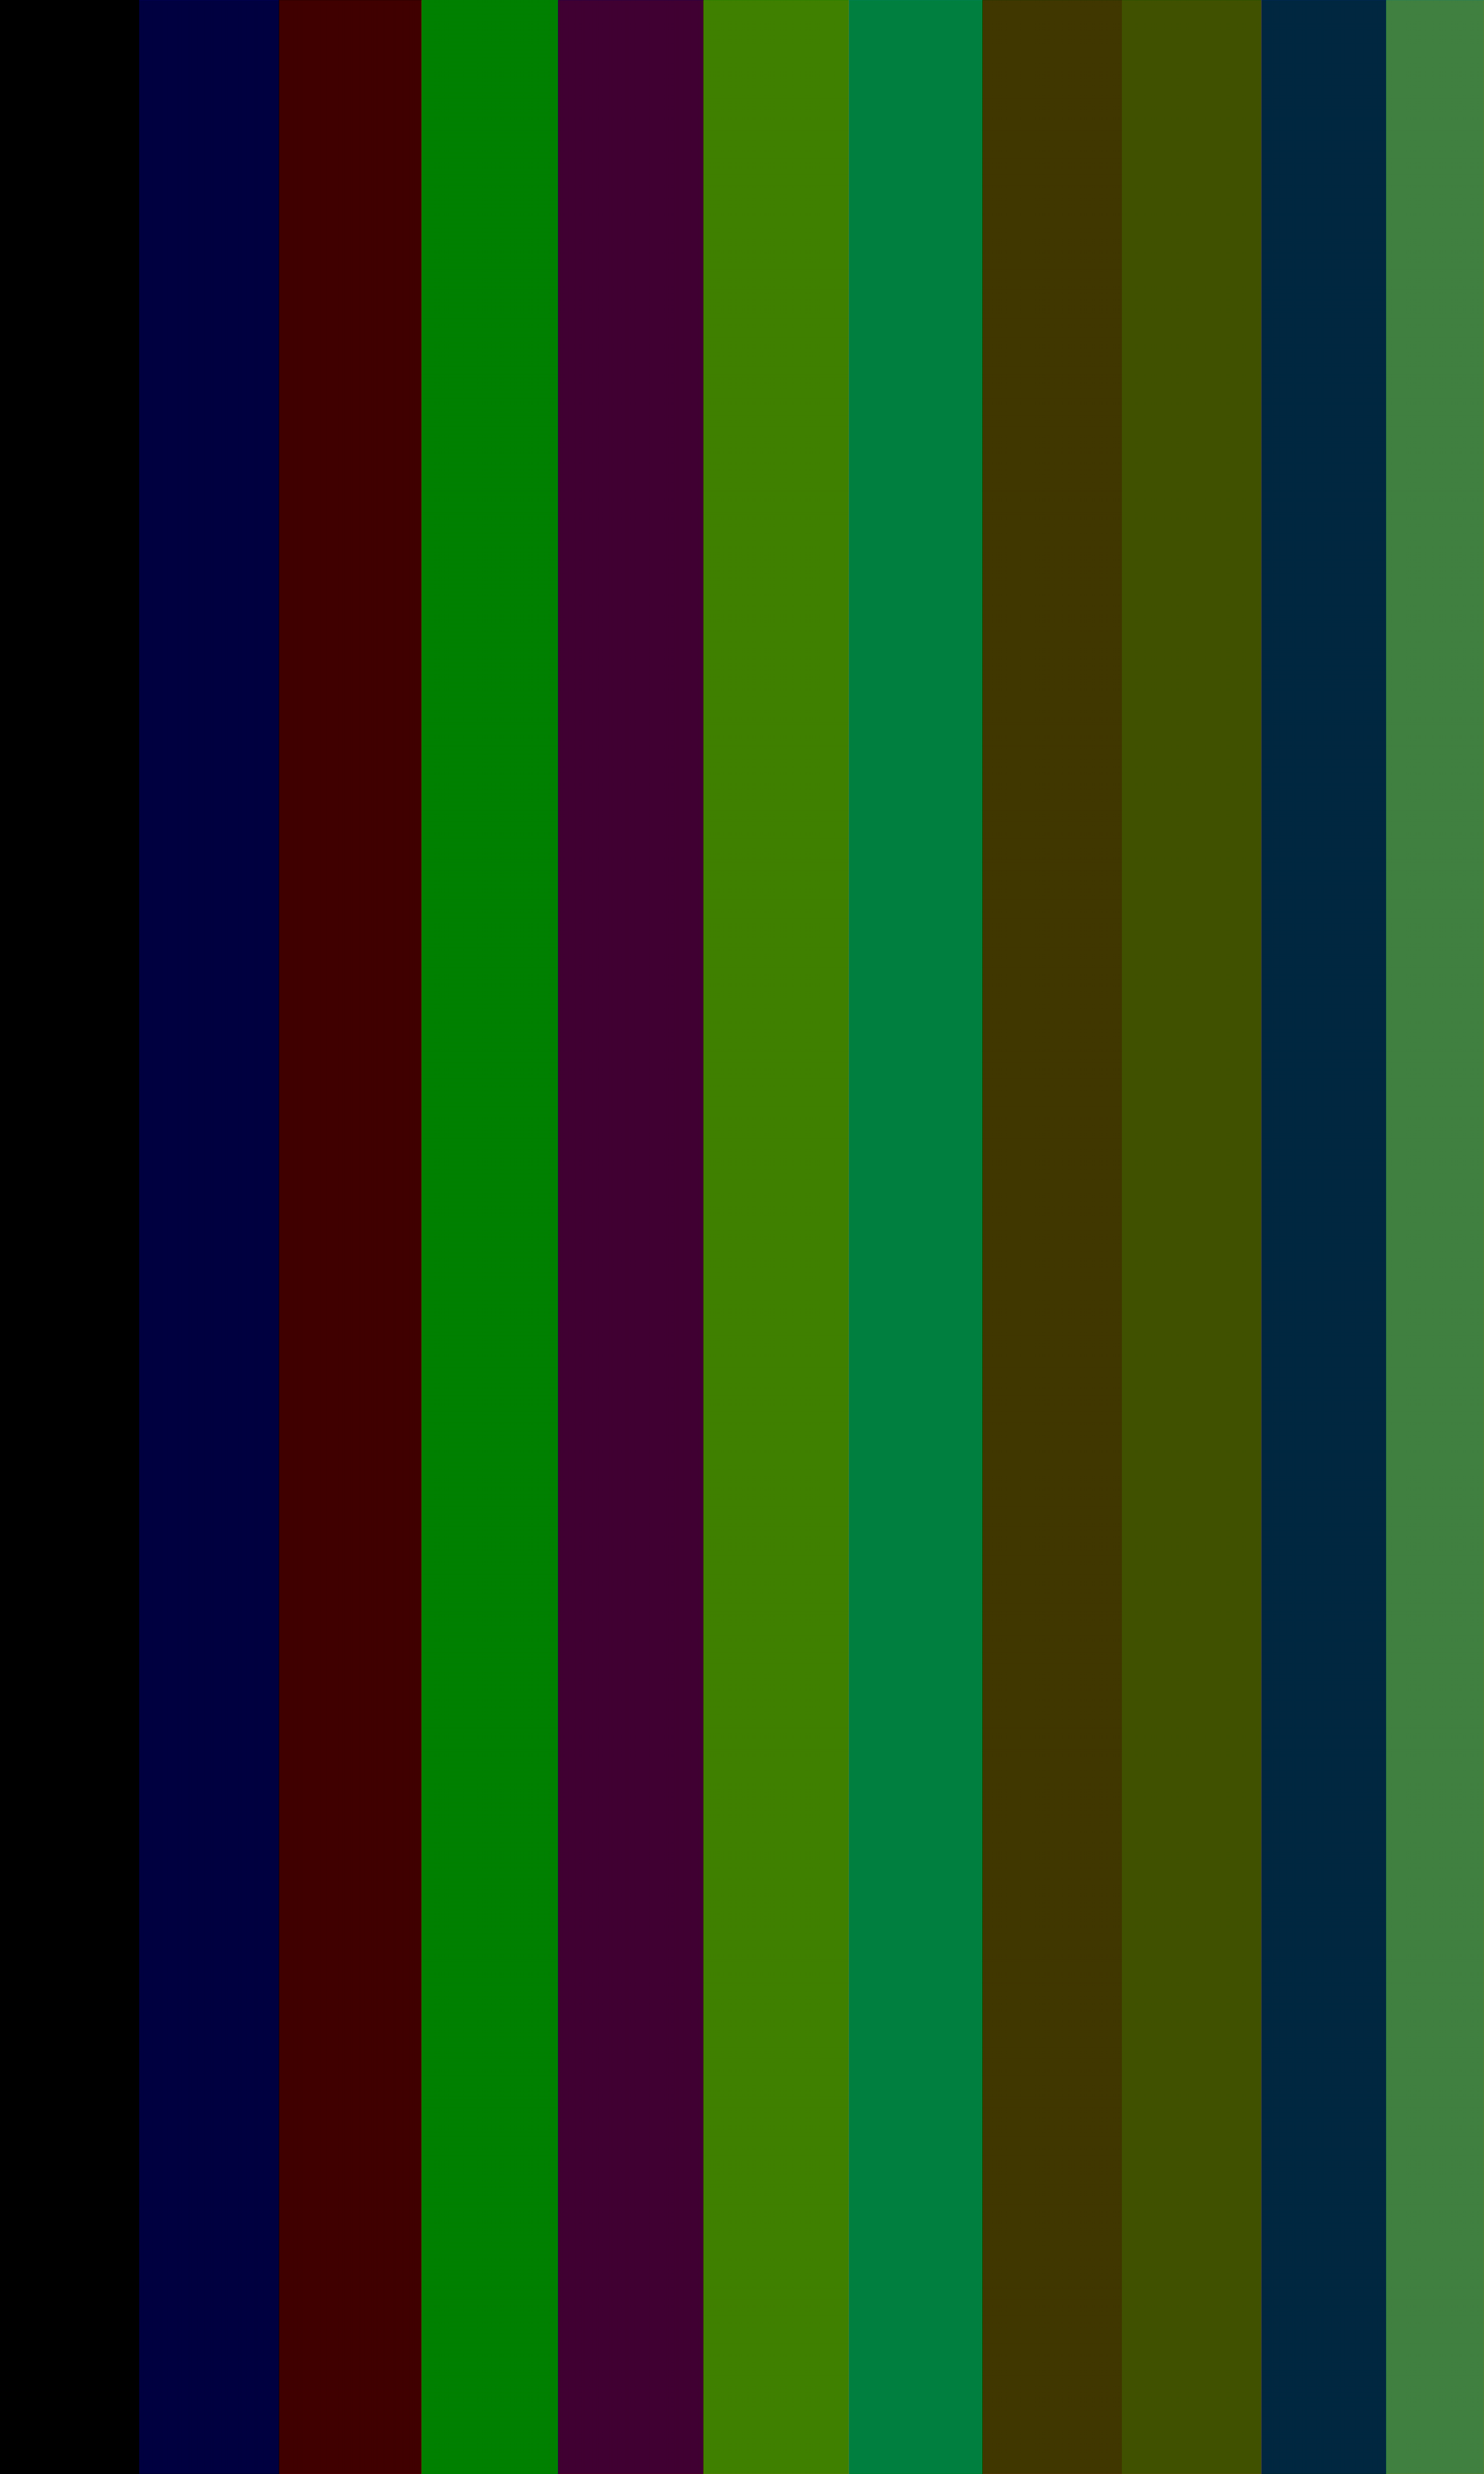
\includegraphics[scale=0.08]{imagenes/colores_bayer.png}
       \caption{Bayerizada}\label{fig:awesome_image1}
        \end{center}
\endminipage\hfill 
\end{figure}
\newpage
\begin{figure}[!htb]
\minipage{0.5\textwidth}
\begin{center}
    
\includegraphics[scale=0.08]{imagenes/colores_demosicing_bilineal.png}
    \caption{Bilineal }
 \end{center}
\endminipage
\minipage{0.5\textwidth}
\begin{center}
    
\includegraphics[scale=0.08]{imagenes/colores_demosicing_quality.png}
    \caption{High Quality}
        \end{center}
\endminipage\hfill
\end{figure}
\newpage
\begin{figure}[!htb]
\minipage{0.5\textwidth}
\begin{center}
    
\includegraphics[scale=0.08]{imagenes/colores_demosicing_spline.png}
    \caption{Directional}
        \end{center}
\endminipage
\minipage{0.5\textwidth}
\begin{center}
    
\includegraphics[scale=0.08]{imagenes/colores_demosicing_vecino.png}
    \caption{Vecinos}
 \end{center}
\endminipage
 
\end{figure}
\newpage

Efectivamente a primera vista parecería que todas dieran lo mismo. Pero veamos que si le hacemos zoom, no es así.
\begin{figure}[!htb]
\minipage{0.5\textwidth}
\begin{center}
    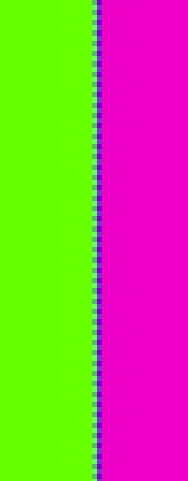
\includegraphics[scale=0.6]{imagenes/colores_bilineal_zoom.jpg}
    \caption{Bilineal Zoom}
        \end{center}
\endminipage
\minipage{0.5\textwidth}
\begin{center}
    
\includegraphics[scale=0.6]{imagenes/colores_hq_zoom.jpg}
    \caption{Bilineal Zoom}
        \end{center}
\endminipage 
\end{figure}
\begin{figure}[!htb]
\minipage{0.5\textwidth}
\begin{center}
    
\includegraphics[scale=0.6]{imagenes/colores_directional_zoom.jpg}
    \caption{Directional Zoom}
        \end{center}
\endminipage
\minipage{0.5\textwidth}
\begin{center}
    
\includegraphics[scale=0.6]{imagenes/colores_vecinos_zoom.jpg}
    \caption{Vecinos Zoom}
        \end{center}
\endminipage 
\end{figure}

Como supimos el algoritmo directional y el bilineal tuvieron pequeños errores en los bordes. Podemos observar que en esos casos entre el verde y el violeta parece haber como una `cosedura', la misma se repite en todos los bordes de la imagen. Estas diferencias imperceptibles por el tamaño de la imagen a primera vista pueden ser efectivamente comprobadas mediante un análisis de calidad objetivo. 

PSNR 41.14 con bilineal
PSNR 39.67 con quality
PSNR 48.13 con directional
PSNR 48.13 con vecinos

tiempos:

\subsection{Imágen 9}
\begin{figure}[h!]

       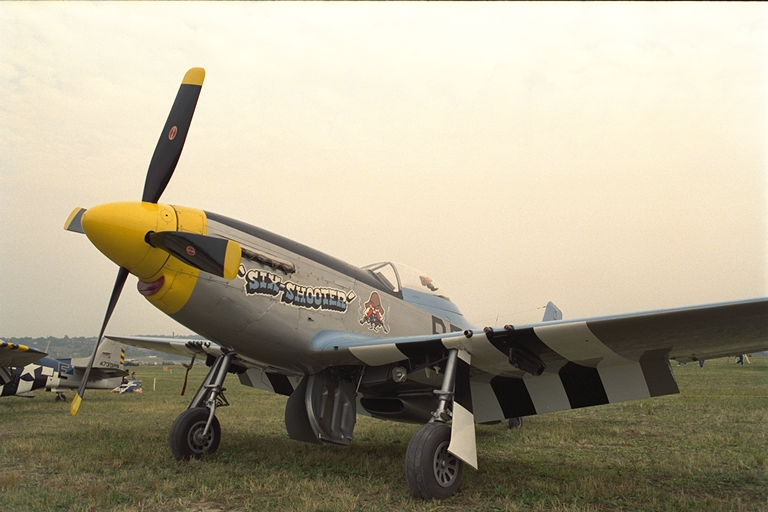
\includegraphics[width=0.5\textwidth]{imagenes/img9.png}
           \hfill
        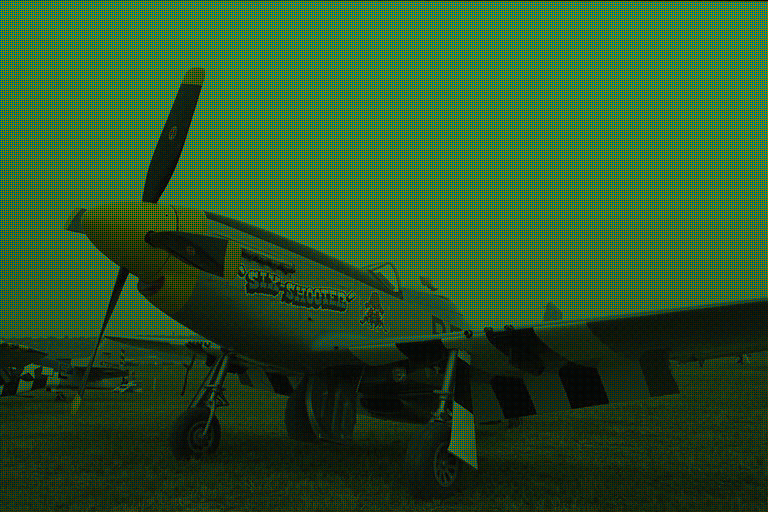
\includegraphics[width=0.5\textwidth]{imagenes/img9_bayer.png}

\end{figure}

\begin{figure}[h!]

       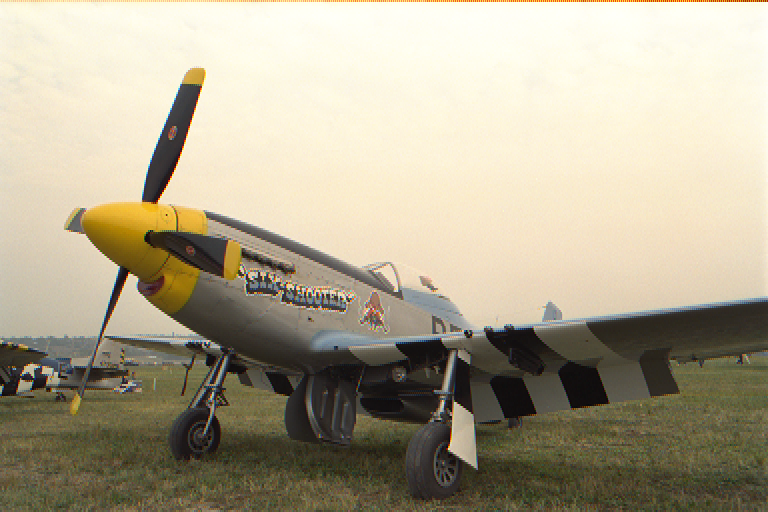
\includegraphics[width=0.5\textwidth]{imagenes/img9_demosicing_vecino.png}
           \hfill
        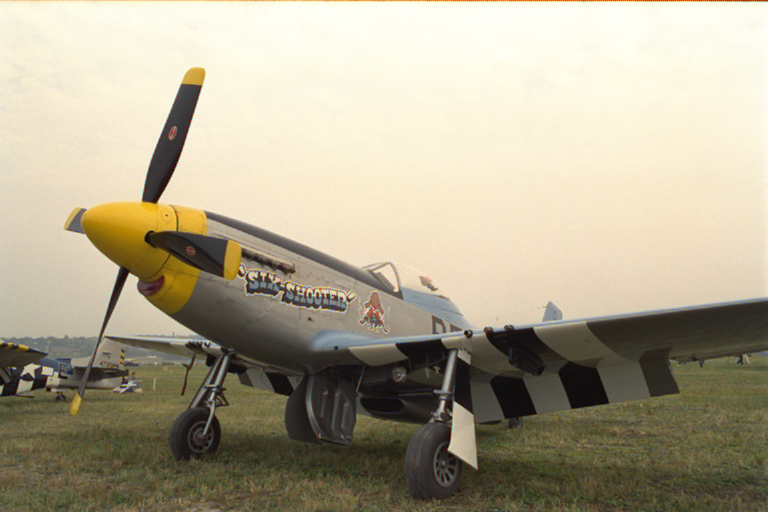
\includegraphics[width=0.5\textwidth]{imagenes/img9_demosicing_bilineal.png}

\end{figure}

\begin{figure}[h!]

       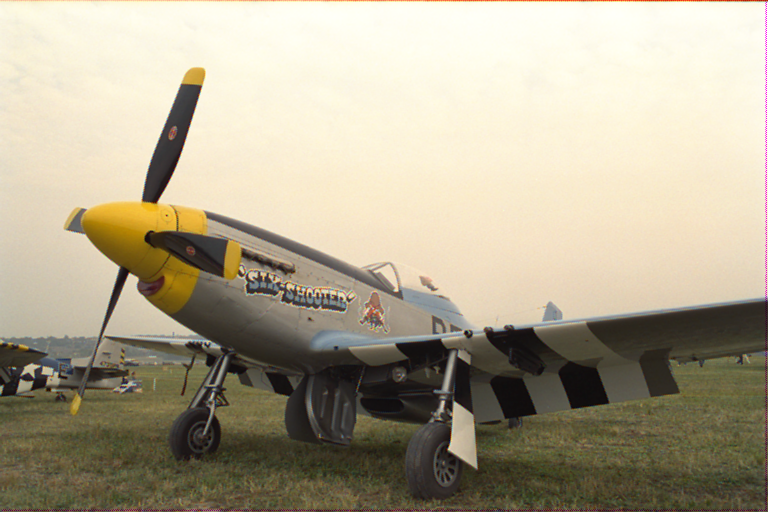
\includegraphics[width=0.5\textwidth]{imagenes/img9_demosicing_spline.png}
           \hfill
        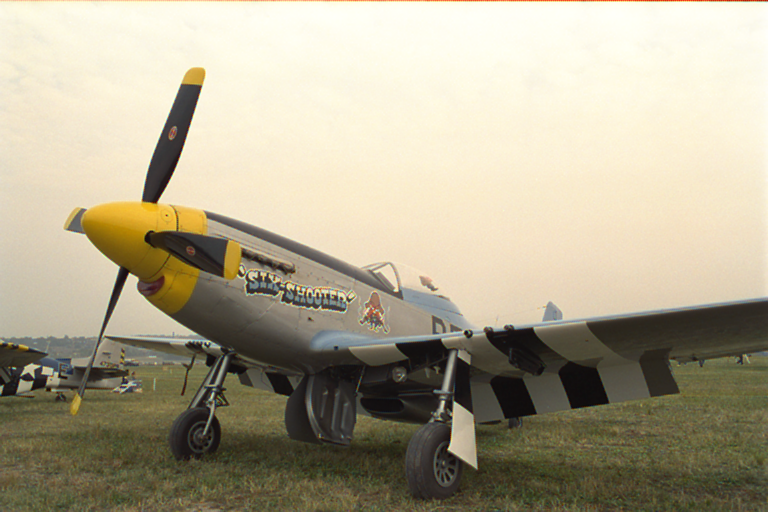
\includegraphics[width=0.5\textwidth]{imagenes/img9_demosicing_quality.png}

\end{figure}
\subsection{Comparación de tiempos}

En esta sección presentaremos una comparativa entre los tiempos que tarda cada algoritmo a medida que aumenta el tamaño de la imagen. Para tal fin testamos cada algoritmo con imágenes cuadradas generadas aleatoriamente que van aumentando su tamaño, y creemos que es una forma correcta de comparar los tiempos ya que la complejidad de cada algoritmo es independiente de la información que tenga la imagen, pero dependiente del tamaño.

\begin{figure}[h!]

       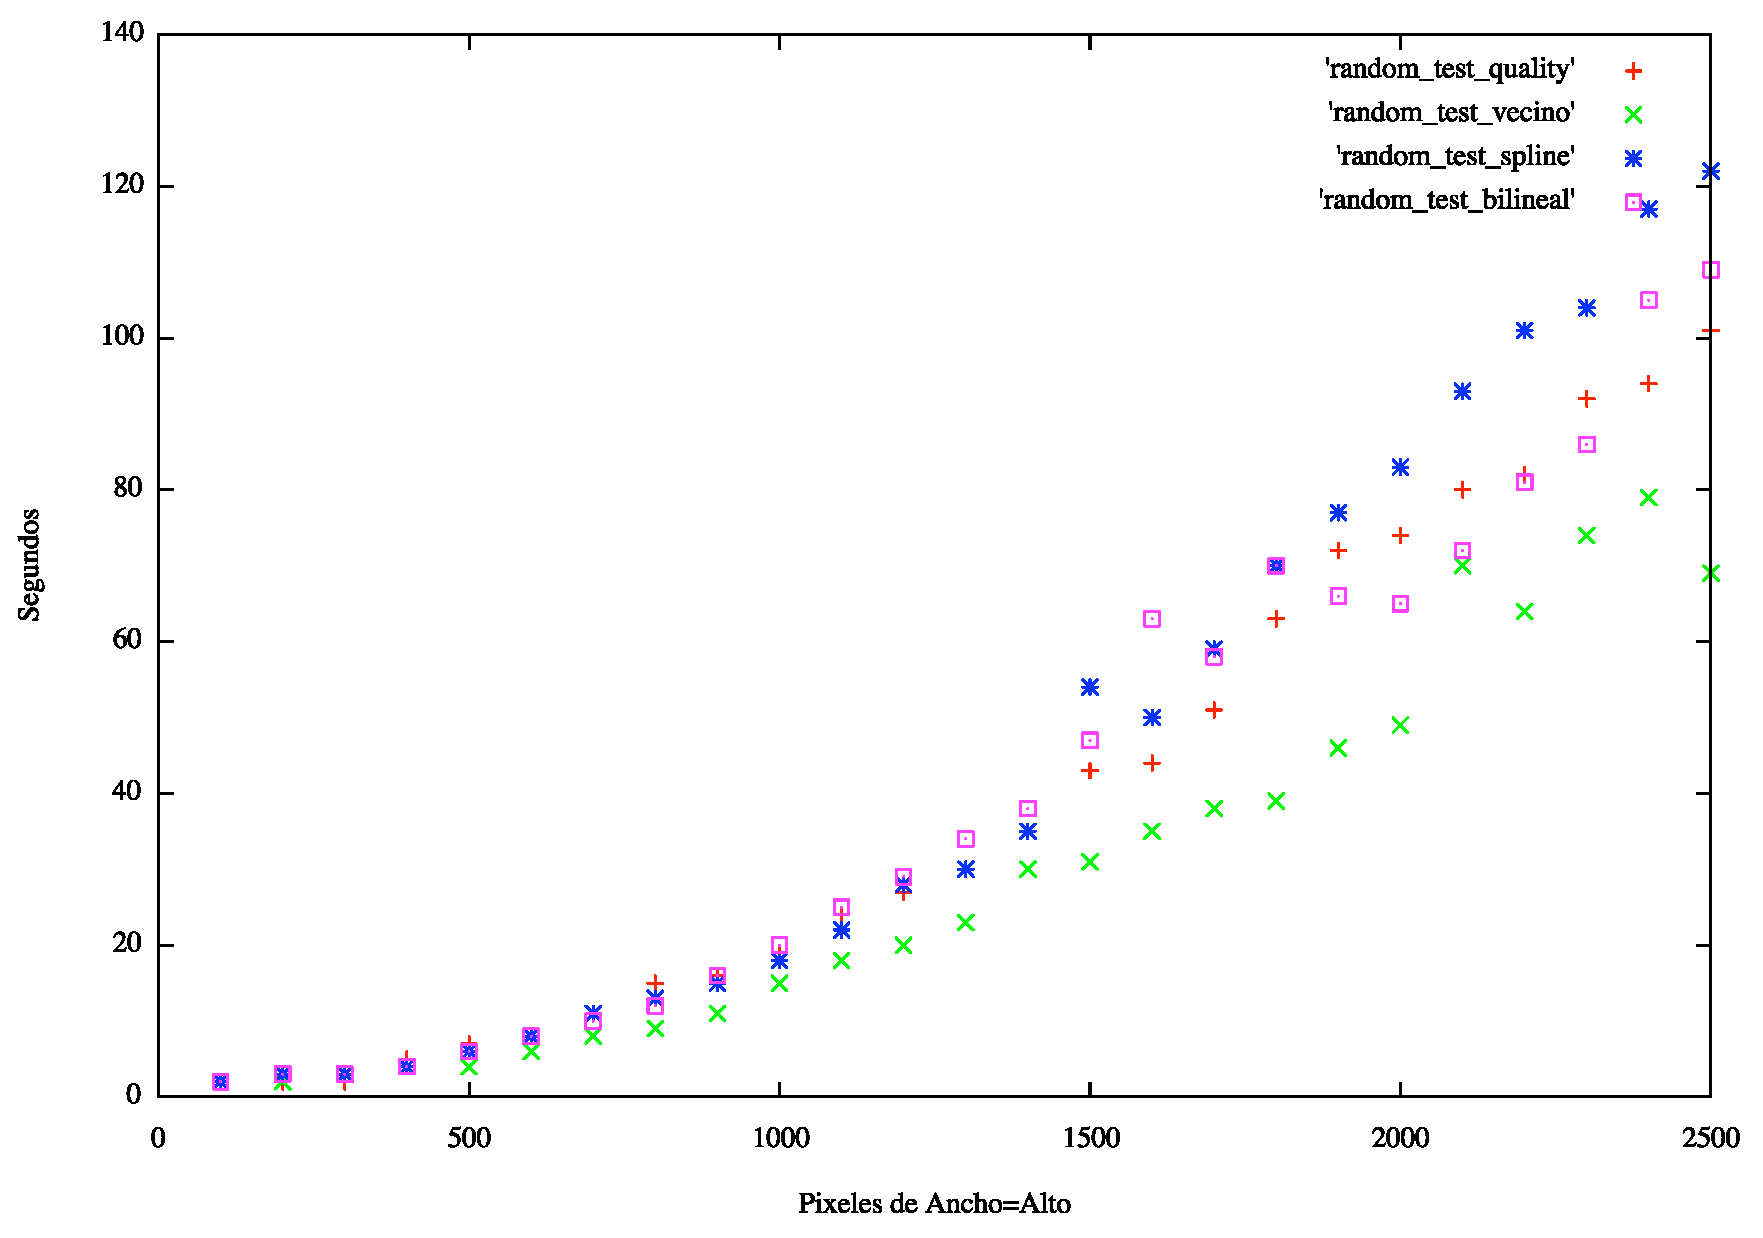
\includegraphics[width=1\textwidth]{imagenes/tiempo_algoritmos_random.pdf}
           

\end{figure}





